% 2018 天津文科第11题正方体四棱锥示意图（据固定源第1页重绘）
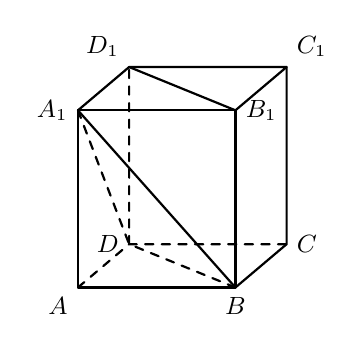
\begin{tikzpicture}[line cap=round, line join=round, thick, every node/.style={font=\small}]
  \coordinate (A) at (0,0);
  \coordinate (B) at (2,0);
  \coordinate (C) at (2.65,.55);
  \coordinate (D) at (.65,.55);
  \coordinate (A1) at (0,2.25);
  \coordinate (B1) at (2,2.25);
  \coordinate (C1) at (2.65,2.8);
  \coordinate (D1) at (.65,2.8);
  % 正方体可见外棱
  \draw (A)--(B)--(B1)--(A1)--cycle;
  \draw (A1)--(D1)--(C1)--(B1);
  \draw (B)--(C)--(C1);
  % 隐藏棱
  \draw[dashed] (A)--(D)--(C) (D)--(D1);
  % 四棱锥 A1-BB1D1D 棱
  \draw (B1)--(D1) (A1)--(B);
  \draw[dashed] (A1)--(D) (B)--(D);
  \node[below left] at (A) {$A$};
  \node[below] at (B) {$B$};
  \node[right] at (C) {$C$};
  \node[left] at (D) {$D$};
  \node[left] at (A1) {$A_1$};
  \node[right] at (B1) {$B_1$};
  \node[above right] at (C1) {$C_1$};
  \node[above left] at (D1) {$D_1$};
\end{tikzpicture}
